\documentclass[12pt, twoside]{article}
\usepackage[letterpaper, margin=1in, headsep=0.5in]{geometry}
\usepackage[english]{babel}
\usepackage[utf8]{inputenc}
\usepackage{amsmath}
\usepackage{amsfonts}
\usepackage{amssymb}
\usepackage{tikz}
%\usetikzlibrary{quotes, angles}

\usepackage{graphicx}
\usepackage{enumitem}
\usepackage{multicol}

\usepackage{fancyhdr}
\pagestyle{fancy}
\fancyhf{}
\renewcommand{\headrulewidth}{0pt} % disable the underline of the header

\fancyhead[RE]{\thepage}
\fancyhead[RO]{\thepage \\ Name: \hspace{3cm}}
\fancyhead[L]{BECA / Dr. Huson / 10th Grade Geometry\\* Unit 7: Analytic Geometry Review\\13 February 2019}

\begin{document}
\subsubsection*{Homework: Completing the square}
  \begin{enumerate}

    \item Complete the t-chart for $x=0,1,2,3,4,5,6$, then plot the points on the grid below.

        \[y = x^2-6x+5\]

        Draw a smooth curve through the points, and label the parabola with its equation.
      \begin{center} %4 quadrant regents grid w T-Chart
      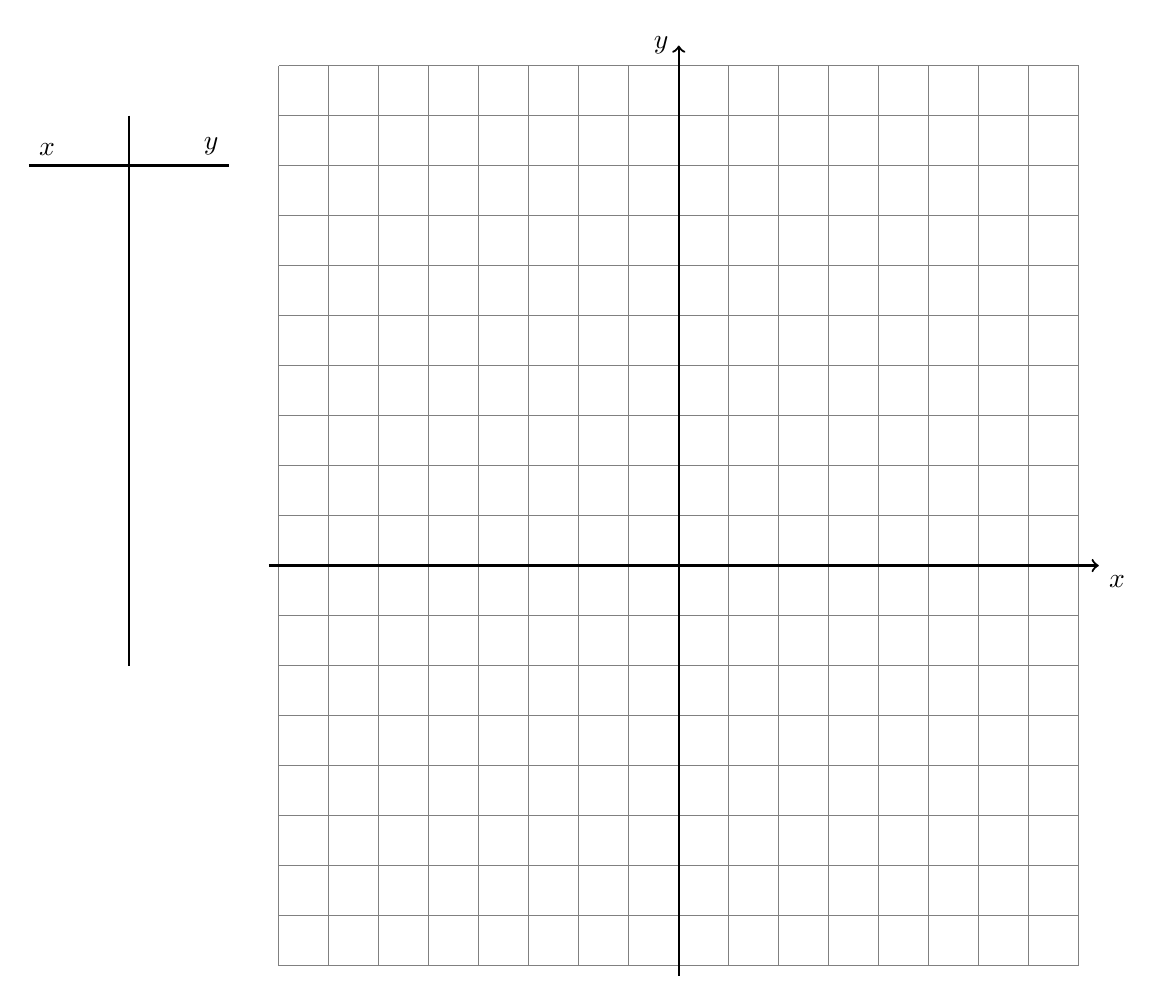
\begin{tikzpicture}[scale=.635]
        \draw [help lines] (-6,-8) grid (10,10);
        \draw [thick, ->] (-6.2,0) -- (10.4,0) node [below right] {$x$};
        \draw [thick, ->] (2,-8.2)--(2,10.4) node [left] {$y$};
        \draw [thick] (-11,8) node[above right]{$x$} --(-7,8) node [above left]{$y$};
        \draw [thick] (-9,9)--(-9,-2);
      \end{tikzpicture}
      \end{center}

    \begin{enumerate}
      \item Mark the $x-$ and $y-$intercepts with their values.
      \item Mark the vertex on the graph as an ordered pair.
      \item Write down the equation of the parabola in vertex form. \vspace{1.5cm}
      \item Explain how this equation could have been derived by completing the square.
    \end{enumerate}



\newpage

  \item Complete the square by adding a constant, then factor as a binomial squared.
    \begin{enumerate}
      \item Example: $x^2+6x \rightarrow$ \qquad $x^2+6x+9=(x+3)^2$
      \item $x^2+4x \rightarrow$
      \item $x^2+14x \rightarrow$
    \end{enumerate}

  \item Simplify each radical
    \begin{enumerate}
      \item Example: $\sqrt{12} \rightarrow$ \qquad $=2\sqrt{3}$
      \item $\sqrt{20}$
      \item $\sqrt{18}$
      \item $\sqrt{75}$
    \end{enumerate}


  \item Graph and label the two equations. Mark their intersection as an ordered pair.

    \begin{multicols}{2}
      $y = 2x-7$ \\
      $2x+4y = 12$
    \end{multicols}
    Are the lines parallel, perpendicular, or neither? Justify your answer.
    \vspace{1.cm}

    \begin{center} %4 quadrant regents grid w T-Chart
    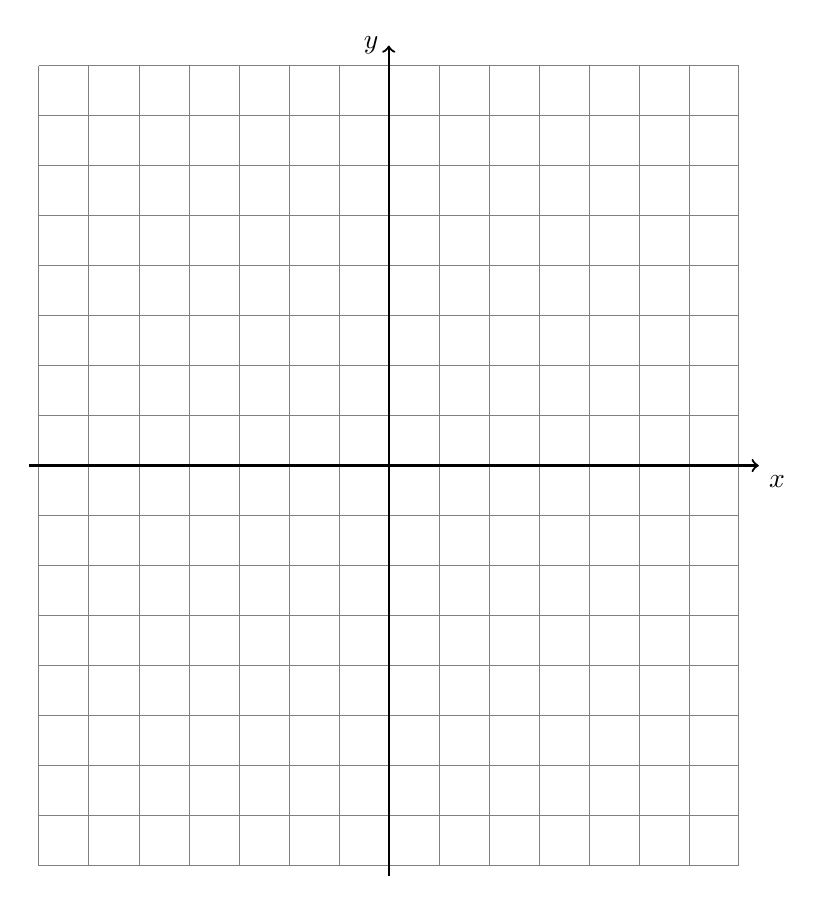
\begin{tikzpicture}[scale=.635]
      \draw [help lines] (-7,-8) grid (7,8);
      \draw [thick, ->] (-7.2,0) -- (7.4,0) node [below right] {$x$};
      \draw [thick, ->] (0,-8.2)--(0,8.4) node [left] {$y$};
    \end{tikzpicture}
    \end{center}

  \end{enumerate}

  \end{document}
